\chapter{State of the Art: Optimal path planning for autonomous robots}

\renewcommand{\chaptername}{Chapter}

\section*{Introduction}

The intralogistics sector is undergoing a significant transformation due to the 
integration of digital tools such as connected industries and robotics. The cluttered 
and highly dynamic nature of this environment makes it challenging to successfully 
implement robotic solutions.

The first steps in digitalizing logistic processes with robots involved the use of 
Automated Guided Vehicles (AGVs). First introduced in 1955, AGVs perform tasks like 
material handling. AGVs are managed by top-level software that handles task planning, 
providing the vehicles with intermediate waypoints to navigate from start to end points \cite{R7}. 

However, the decentralized decision-making approach of AGVs makes them 
unresponsive to changes in their environment. For example, AGVs localize themselves 
using specific and precise anchors physically located in their workspace. 

This localization mechanism helps them follow the assigned path. As a result, even 
a simple environmental change of the dispositionsrequires an update of the measurements 
and maps on  which the planning is based. Another example is that an AGV is unable to plan and 
execute a solution if it encounters an obstacle on its way to the goal or it arrives at a shifted 
destination. In such cases, 
the AGV’s reaction is to stop and wait for top-level instructions \cite{R8}. This behavior 
decreases productivity and disrupts the planned sequence of tasks until an intervention is managed.

To overcome these disadvantages of AGVs, Autonomous Mobile Robots (AMRs) were introduced. 
AMRs are equipped with a decentralized control system, enhanced perception of their 
surroundings through more complex hardware, and advanced software to manage and integrate 
these hardware additions (Figure \Ref{AMR-VS-AGV}).

\begin{figure}[H]
    \begin{center}
       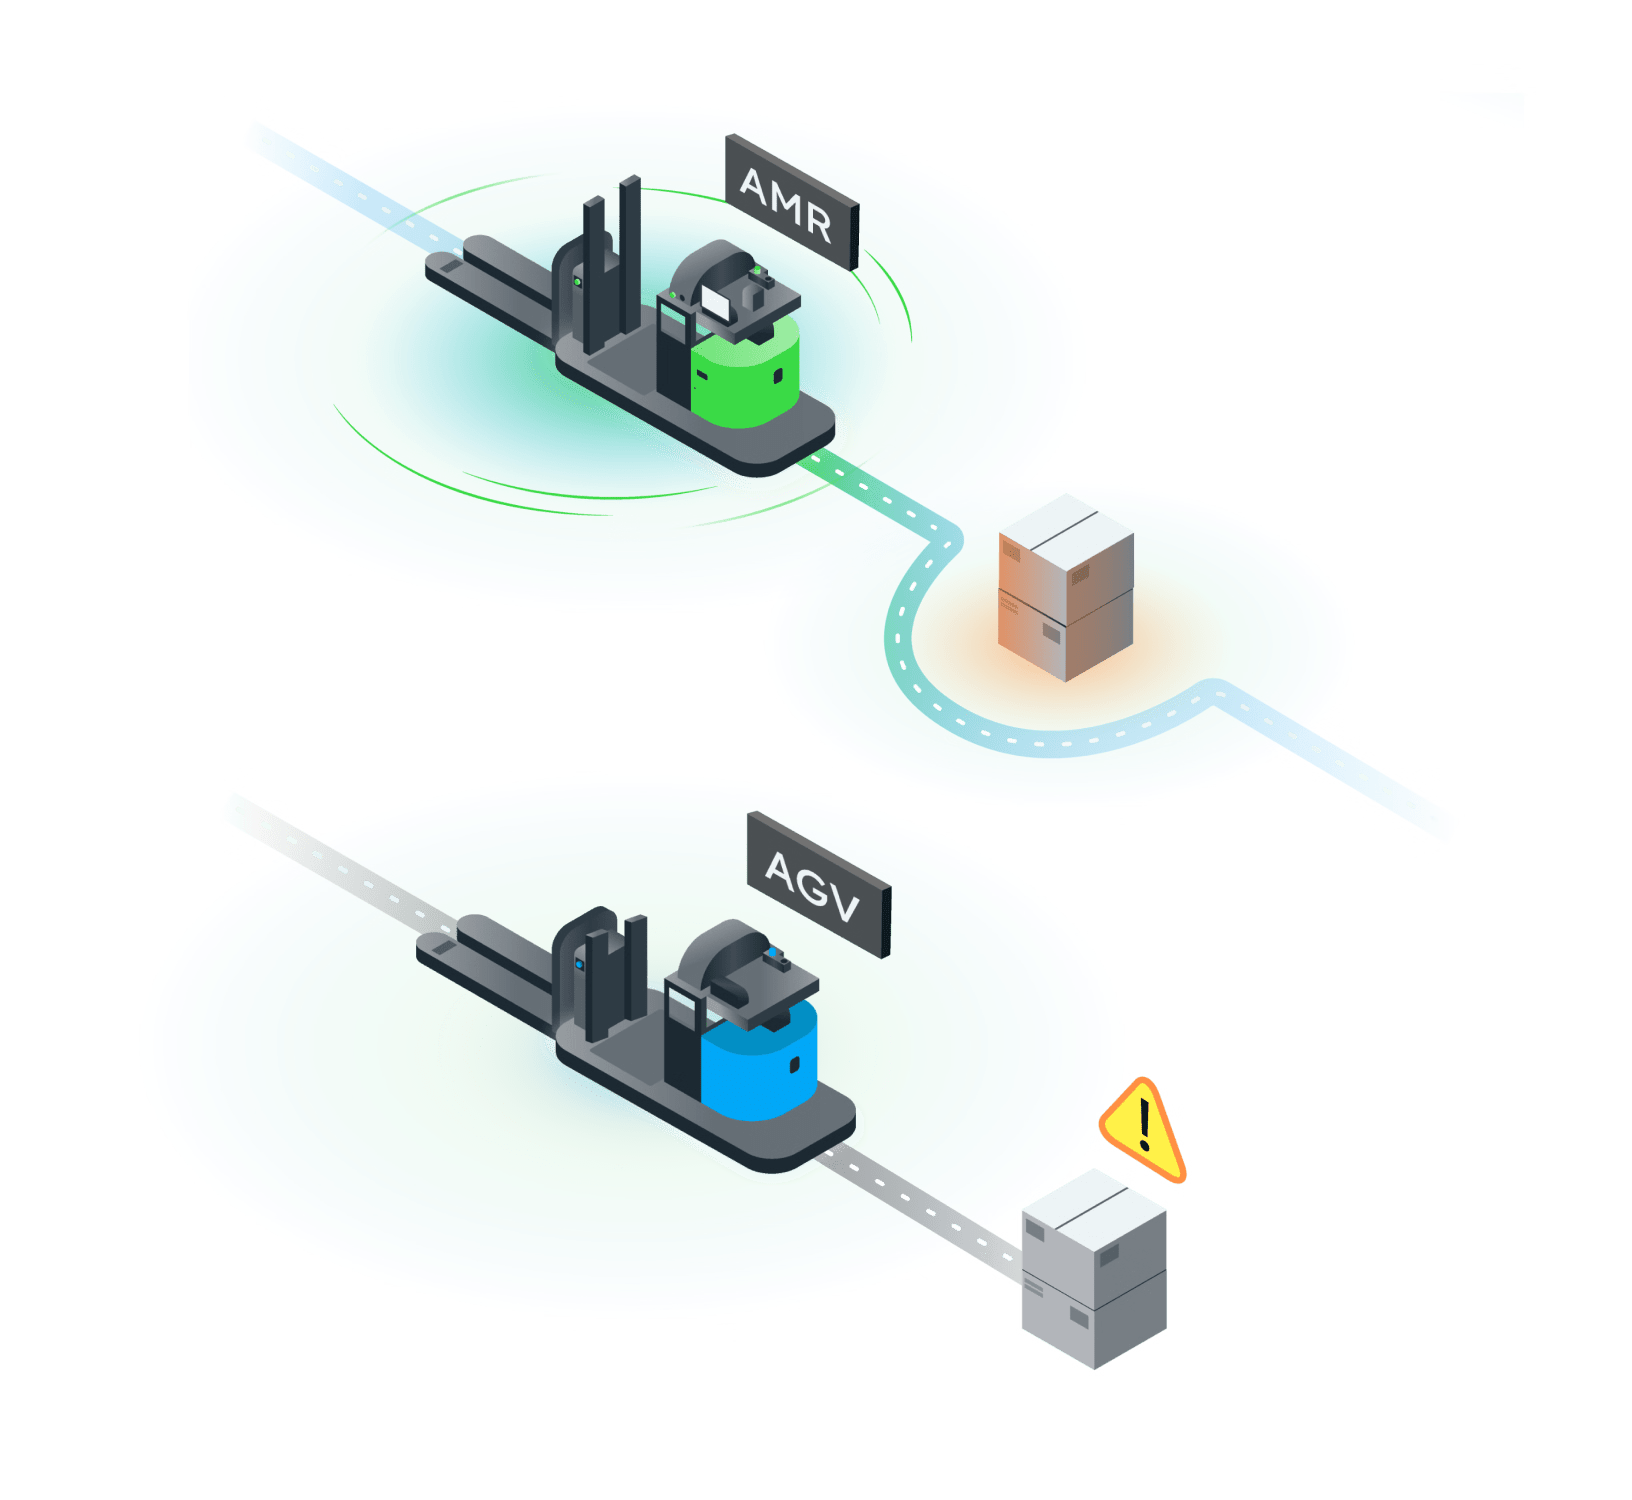
\includegraphics[width=4in]{images/Chap1/AMR-VS-AGV.png}\\
       \caption{AMR and AGV behaviors at presence of an obstacle \cite{R9}}
       \label{AMR-VS-AGV}
       \end{center}
\end{figure}

In addition, they grant a fast integration into new environments due to smart perception 
and recognition technologies. AMRs use this data as input to smart algorithms that 
enable it to plan its missions, navigate to its destination, avoid collisions, and 
execute missions all while collaborating with humans in the working space. The 
Autonomous vehicles do not require an automation expert or a roboticist’s presence to 
be configured or to deal with complex situations. It is able to solve such situations 
individually due to the scalable software that it has on board.

On the one hand, this evolution enables AMRs to navigate more dynamically and adaptively 
within intralogistics environments, improving overall efficiency and responsiveness. 
On the other hand, the level of flexibility that AMRs brings important safety and 
efficiency considerations \cite{R7}.

One of the main challenges is developing the navigation mechanisms. In a logistics 
environment, it is crucial to comply with the nature of the workspace. The AMR should 
recognize the location of materials to be handled and be able to navigate to and from 
those locations to next missions. Building a flexible and efficient solution requires a 
deep understanding of the situations and special cases that the vehicle may encounter 
and a study about how to create scalable solutions for such events.  

Before diving into the methodologies and technologies used to address this thesis’ 
topic, it is relevant to examine the related works. This research will serve later in 
the thesis as a guiding outline. Literature helps to investigate the level of progress that 
other researchers reached in similar topics, prevents re-invention of existing concepts, 
and pushes to ethically exploit the developed technologies. For this thesis, it is 
important to deeply examine the research papers and scientific resources to build a 
solid foundation of knowledge, identify the gaps in some studies, and propose novel 
solutions.  

In this context, this state-of-the-art report, delves 
into pathplanning and near-field path planning for mobile robots 
in general and for intralogistics AMRs specifically. Then, it examines possible 
solutions for path creation and generation. Afterwards, 
it studies the decision-making science approaches that can be used to evaluate and 
optimize path suggestions. Finally, this chapter 
outlines the methodology to be followed throughout this scientific work(Figure \ref{mindmap}).

\begin{figure}[H]
    \begin{center}
       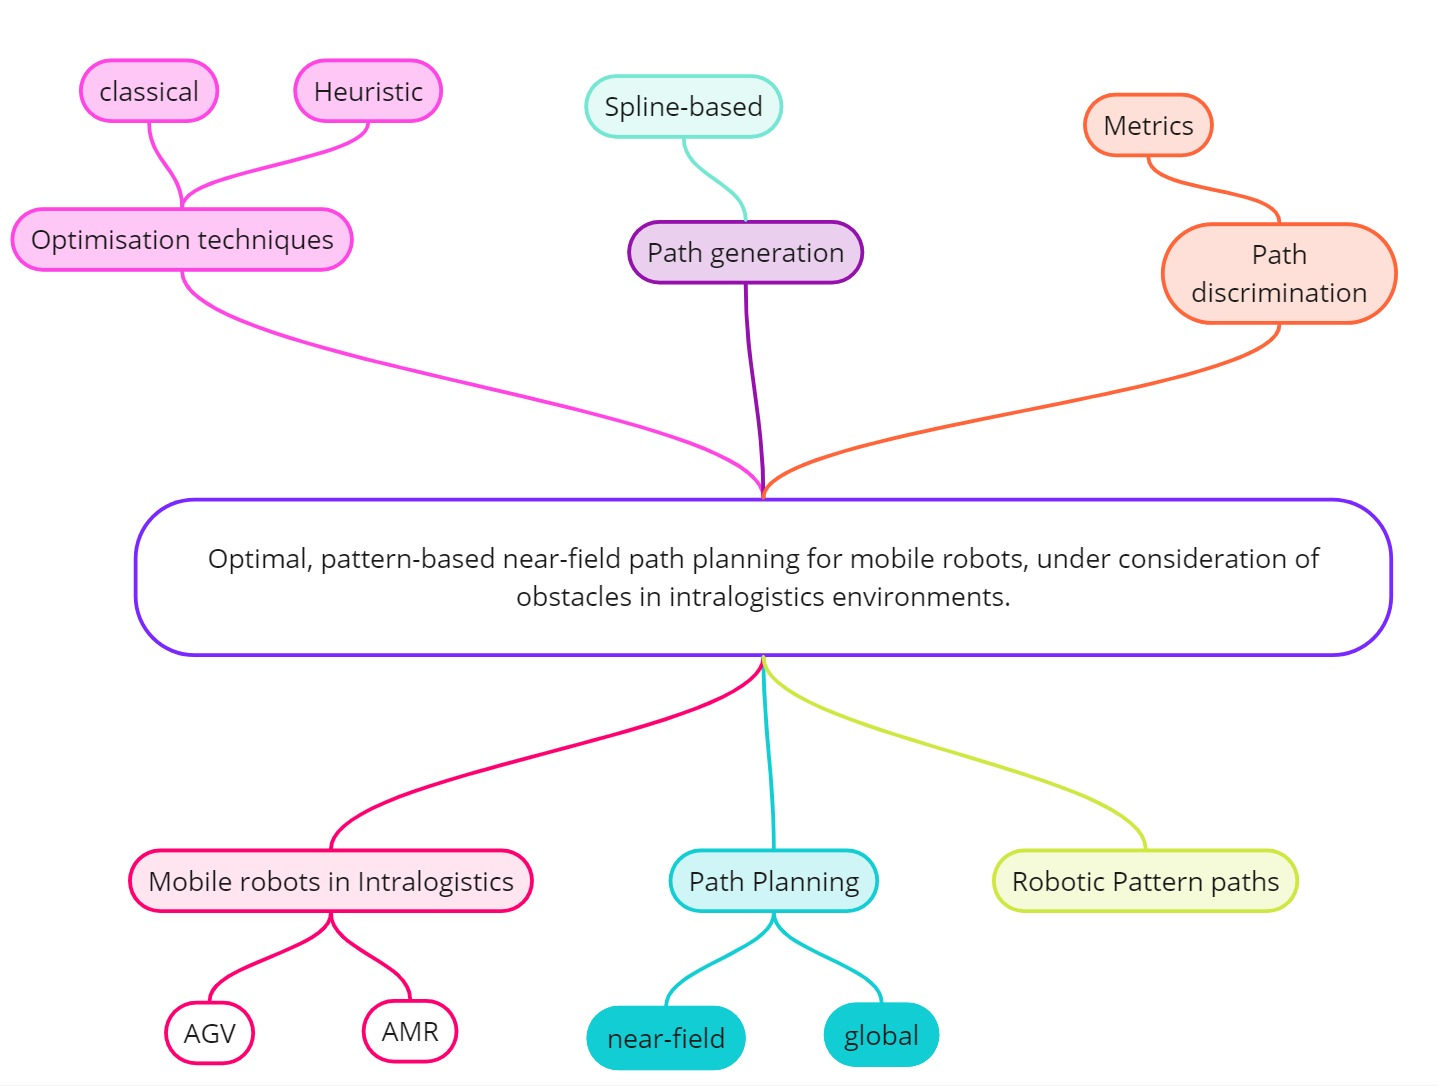
\includegraphics[width=5in]{images/Chap1/Fig1.jpg}\\
       \caption{Mind map of the key topics}
       \label{mindmap}
       \end{center}
\end{figure}

\newpage
\section{Path Planning}
This section will dive into the path planning state of the art: presenting its promising 
opportuniities and current challenges, detailing the different approaches, and discussing
their efficiency and compatibility with the problem statement.

\subsection{Path Planning for autonomous robots: Opportunities and challenges}

Path planning for mobile robots involves creating and generating efficient routes 
for the robot to travel from a starting position (A) to a target position (B), 
ensuring minimal time and travel distance while avoiding collisions with nearby objects \cite{R7}.

In complex environments, it is challenging for robots to move randomly and fulfill 
their missions. However, with appropriate input from various sensors, such as laser 
scanners, cameras, and LiDAR, robots can perceive their surroundings and plan the right path
accordingly. The innovation in hardware made navigation flexibility and autonomous recovery 
after failure possible\cite{R7}.

The application areas of path planning for autonomous mobile robots are factories and warehouses, 
healthcare institutions, hotels and restaurants, and domestic areas.
The relevance of efficient path planning, mainly in the intralogistics sector, is derived from the constant need 
of optimizing material flow, productivity rates, and cost effectiveness. Path planning is very promising to reduce
travel time and distances when moving goods and thus, improving overall operational costs. 

In those dynamic environments, operators and employees are moving around, goods and pallets are 
being transported or stocked, and materials must be handled safely and carefully.
Flexibility in routing and planning, enables the autonomous vehicles to always drive the optimal path
based on the space settings. The benfits here include:
\begin{itemize}
    \item Independence from Human intervention -AMRs do not require assistance, unike AGVs \cite{R7}.
    \item Respect of safey standards through developed vision and recognition: critical personnel safety protection,
    preserving the handled goods, 
    manufacturing systems, storage material or other vehicles.
    \item Reduced energy consumption thanks to optimal: smooth and short paths that respect the vehicles' kinematics
    and allocated task and travel time.
    \item Robustness and responsiveness thanks to decentralized decison making: enables fast recovery after failure \cite{R7}.
    \item Alignment with real-world applications and the growing demand for automation in logistics due to e-commerce 
    growth and supply chain complexities.
\end{itemize}

Efficient path planning is essential for ensuring the safe handling of objects in the environment. 
In intralogistics, the materials being handled—whether goods, manufacturing systems, storage 
shelves, or other vehicles—are valuable and must be treated with care. Moreover, safety is a 
critical concern, especially when human safety and protection are involved. To pass quality 
tests, autonomous forklifts must meet personal safety requirements. These requirements include, 
but are not limited to, maintaining a safe distance from both static and dynamic objects and 
people, as well as detecting surroundings at any height and time. By following an efficient 
path, overall productivity increases since operations are repeated many times throughout the 
day. An efficient path optimizes both length and smoothness, thereby reducing travel time. 
Additionally, efficient path planning conserves the truck's energy, reducing the frequency of recharging.

Autonomous robots, as the name suggests, are 
standalone systems that must compile and process such input and generate, through algorithms, 
efficient paths. Path planning serves as the crucial 
link between the robot’s sensor input and its motion control \cite{R10}.

Literature and scientific studies differentiate between two main types of path planning: 
global and local path planning. Global planning involves finding an optimal path from 
the start to the target position based on sensor input within a known, static environment, 
whereas local planning focuses on real-time obstacle avoidance, typically used while 
moving to avoid dynamic obstacles \cite{R11}.

%challenges
More that 60 years have elapsed since "Shaky" the first wheeled robot was running it first tests
in Stanford University' labs. However, most of the robotic related topic are still being researched and improved.
Dealing with all the aspects and challenges that robotics comes with can be very intricate. One of the major 
topics posing challenges to researchers is path planning. 
In a research by S. H. Tang et al. \cite{R20}, the authors reviewed recent path planning approaches and challenges
in dynamic unkown environments. 
% safety
Saftey in path planning was the main concern for 29 \% of the reviewed studies. Navigating efficient 
paths while avoiding collisions is challenging to accomplish. Collision avoidance is tightly related to perception 
input through sensors, analysis and use of the data. While it may seem simple for the robots to correctfully analyze 
and recognize the objects around them, in reality, detailed understanding is not possible \cite{R21}. Issues are 
related to the accuracy of the sensors and the robustness of the algorithms. 
It is expected from the robot to 
preceive of the obstacles just like humans do, recognizing 3d shapes, dimensions, depth, direction and velocity, 
but from the 
robot's perspective, it is only able to recognize the outer surface that reflects the sensor's signals as shown in
figure \Ref{scamSim}.

\begin{figure}[H]
    \begin{center}
        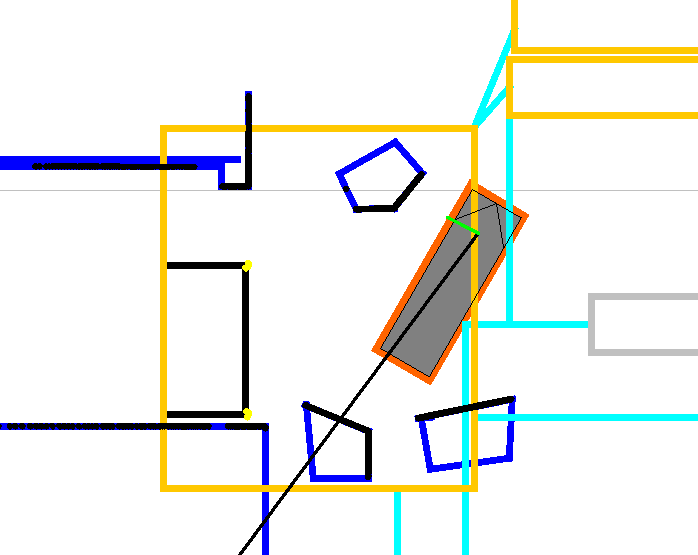
\includegraphics[width=4in]{images/Chap1/scan.png}\\
        \caption{
        Simulation of the robot's perception of surrounding obstacles.
        \newline \textbf{Yellow rectangle:} Station limits
        \newline \textbf{Black rectangle:} Shelf limits: where to pick or to place pallets
        \newline \textbf{In gray:} Robot in simulation
        \newline \textbf{Blue polygones:} Simulated obstacles
        \newline \textbf{Black lines:} Perceived obstacle points}
        \label{scamSim}
        \end{center}
\end{figure}

As a result, algorithms are to compensate this ambiguity by enforcing safety measures like 
keeping the vehicle at a safe distance from the obstacles and deccelerating at the proximity 
of static and dynamic objects to avoid collisions
In addition, this input contains noises and shadows caused by the sensors reflections of other objects
or inaccuracies. 
This makes it challenging to interpret the input and make safe decisions as the built algorithms have to deal 
with the given data
in all cases and detect the inaccuracies and noises. In \cite{R22}, the authors investigate a collision 
avoidance approach 
Beyond that, it is complex to generate feasible solutions in all types of environments,
some planners and algorithms risk stagnating in a local minima and not converging to the optimal routes. 

%Computational intensivity

Besides safety, computational cost is an interesting topic that researches 
are looking at. It is considered as a key metric by scientists to judge if an algorithm will be able to 
accomplish certain tasks within the needed time frame. It accounts for the time and resources consumed
by the algorithm while computing \cite{R24}. In an experiment to compare global motion planners, Heiden et al. use different metrics on which 
they based their comparison. Computation time is one of the considered factors used to discrminate
approaches. They study closely the difference in computation time in different environment scenarios 
besides the effect of certain improvements introduced to the algorithms on the 
computation time. The computational cost is justified by optimizations running on the computed paths like 
path smoothing, 
computing steer functions, and checking for collision possibilities \cite{R23}. In a real time context, it is important to synchronize different tasks, 
analyze massive amounts of data generated by sensors and camera like point clouds and 2d/3d images, 
and compute the required decisions in a reliable and accurate way. As the complexity of the environment 
increases, so does the computational burden, often leading to longer processing times or the need for 
more powerful hardware \cite{R23}.

%smooth paths length and control:
While managing computational costs is crucial, it is equally important to ensure that the paths 
generated are not only computationally efficient but also smooth and short, as these factors 
significantly influence the robot's overall performance and energy consumption.
Given the kinematics of a robot, the destination's location and the clutter in the environment, 
path planners unusually render rough paths. Cusps, which are sudden and sharp direction changes, and high
curvatures of the path are unusual path properties that are hard to drive, energy and time inefficient, 
and require continuous decelerations and accelerations. Long paths are also not favored. While they can be 
necessary to avoid obstacles or to create a smooth path, longer distances result in time consumption and 
extensive energy usage. 
Some path planner include post-smoothing methods that modify the paths after its creation and intervene by
shortening and smoothing paths areas while obstacles. In \cite{R23}, Heiden et al. present various ways 
to implement like using splines, and short-cuts. They conclude that different methods deal with certain 
improvements areas differently. For example, While Splines are outperformed in the curvature and cusps 
areas, they are efficient when it comes to path-smoothning computation time.  

In conclusion, tackling robot path planning requires looking at several improvement
areas at the same time. Through an analysis of \cite {R20}, we can notice that most of the studied approaches 
are effective in particular aspects, but lack optimization in others. This further emphasizes that these 
challenges remain under research and are not yet fully addressed in the literature. While these challenges 
highlight areas needing further exploration, various path planning approaches offer different strategies 
to address them. Understanding these approaches can provide insights into potential solutions and 
advancements in overcoming the existing limitations.


\subsection{Comprehensive Path Planning Approaches}
\subsubsection{Global Path Planning}

At the beginning of the research phase for this thesis, it was important to look at the available types 
of path planning methods. Science generally distinguishes between three general approaches of Global 
Path Planning all having the same aim to plan the path from a start to a goal position within a pre-mapped 
environment:  grid-based methods, sampling-based methods, and artificial intelligence-based methods \cite{R13}. 

Grid-based methods involve discretizing the environment into a grid of cells, where each cell represents 
a small, discrete part of the space. Then, the algorithm visits the grids to decide which cells will 
be used for the path based on the occupancy or cost and calculates the fitness function from start to 
the reached point in A* algorithm for example or from the reached point to the destination for Dijkstra 
Algorithm. While this method seems easy to understand and quite simple to implement, it is 
computationally intensive because of the number of grids to evaluate and the repetitiveness 
and constrained in direction (Figure \Ref{direction possibilities}) 

Sampling-based algorithms do not discretize the entire environment into a grid but instead randomly sample 
the space to construct a path: the samples are distributed in a manner that they avoid the obstacles 
and serve as a roadmap for to create a start-to-end path \cite{R15}. The exact approach to transform the 
roadmap into a continuous path depends on the algorithm like PRM or RRT. 

Sampling-based algorithms present advantages like handling big environments and complex situations, 
however, they can also be computationally intensive and demanding in such situations. 
Figure \Ref{sampling-based} shows the difference in the resulting optimal path in a cluttered environment where with 
1 core the algorithm successfully finds a feasible path, and, as the cores double, the computed path 
improves its quality as the search tree expands. 


\begin{figure}[H]
    \begin{center}
       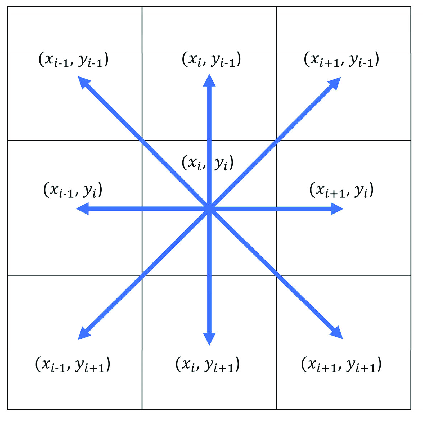
\includegraphics[width=2in]{images/Chap1/8dirs_pathPlan.png}\\
       \caption{8 direction possibilities to move from the current cell to the next cell \cite{R14}}
       \label{direction possibilities}
       \end{center}
\end{figure}

As for artificial intelligence-based methods, also known as heuristic and metheuristic approaches, 
leverage the use of neural networks, machine learning and deep learning, and evolutionary algorithms. 
These methods learn from experience, adapt to changes, and optimize paths in complex environments. 
They are good at handling dynamic and unpredictable scenarios, making them suitable for tasks like 
autonomous driving, robot navigation, and logistics. 


\begin{figure}[H]
    \begin{center}
       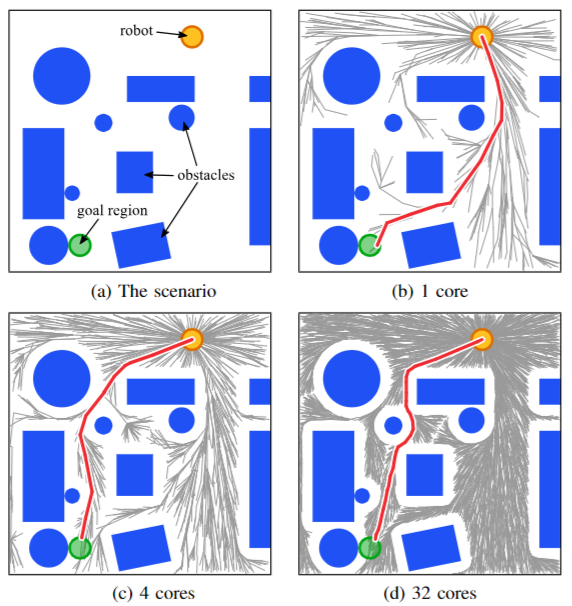
\includegraphics[width=3.5in]{images/Chap1/sampling-based.png}\\
       \caption{8 direction possibilities to move from the current cell to the next cell \cite{R16}}
       \label{sampling-based}
       \end{center}
\end{figure}

To start with, Neural networks (NN) are inspired from the biological harmonious connection of the brain neurons
that gives it the ability to process big amounts of data and generate ideas and decisions and solve problems. 
The NN is built in a way that enables it to get its input in a form of data and process it by learning, improving 
and adjusting the output to the desired results. NN are able to perform Parallel processing: the information is 
transmitted in two
directions to the neuron in the case of Recurrent Neural Networks (RNN) that allows for learning fron current and 
past inputs to the NN. This approach improves the computation time and overall performance. 
The NN is then able to process complex solutions and create paths for difficult environments. 
It is well suited for unpredictable situations as it is built to adapt to the available input and the desired output.
However, it presents a practicality challenge. Althugh the performance an results can be impressive, yet, in a 
real-time context, 
it is hard to rely on solutions that require extensive computational efforts and need long durations to 
process solutions. In addition, the number of neurons and layers have to be scalable and depends closely on the 
level of complexity that the vehicle is to deal with \cite{R12}. 

Fuzzy Logic (FL), on the other hand, is a way of thinking that mimics how humans make decisions, especially when things are unclear 
or uncertain. Instead of working with exact numbers, it uses "fuzzy" terms like "good", "average" or "bad" to make 
decisions. Input numbers are clustered following the fuzzy sets or intervals and assigned a value using membership 
functions. Later the values are interfered and defuzzified to genearte the ouput as a command value. 
In robotics and path planning, FL helps robots navigate by allowing them to handle uncertain situations, 
like avoiding obstacles or finding the best route, even when the environment is not fully known. Instead of needing 
exact data, the robot can employ fuzzy terms like "close" or "far" to understand its surroundings. For example, if an 
obstacle is "somewhat close," the robot can smoothly adjust its path to avoid it. FL also helps the robot choose the best 
route by weighing various factors like distance and safety, even when the information is not perfect. This makes the 
robot better at handling unpredictable environments and making flexible and optimal decisions.
However, one 
disadvantage is that it can be tricky to create the right rules for the robot to follow, and the system can become 
complicated as more rules are added. It may present a scalability problem because in unpredictable and dynamic environments
it is not simple to decide about fixed fuzzy sets that would be practical in all of the cases \cite{R12}.

While Neural Networks and Fuzzy Logic offer powerful approaches for handling uncertainty and complex decision-making, 
another key area in artificial intelligence for path planning is the use of meta-heuristic algorithms.
Meta-Heuristoc algorithms are inspired from biological and natural processes for evolution and survival. 
Unlike NN and FL, that rely on data as input to generate decisions, meta-heuristic algorithms explore the solution
space by evolving random solutions for the problem and optimizing them by rounds until a stopping criterion or set
of criteria is satisfied (see more in section ...: Optimization Algorithms).
Approaches like Genetic Algorithms (GA) have been used for path planning by Ahmed Elshamli et al. \cite{R17}. The The robusteness of their 
solution is the adaption of the solution to dynamic environments. They evolve their GA using variable size chromosomes, where each node 
represents a waypoint of the path, then they measure the quality of each path using an evaluation function. A modified Genetic Approach is then 
applied to each population: Crossover, mutation, \textbf{Repair} infeasible paths, \textbf{Shorten}, then \textbf{Smoothen} 
feasible paths while dynamically checking for new obstacles.
The approach is tested in static and dynamic environments and has achieved proven efficiency when it comes 
to local optima challenges and survivig the best elements of the population. While the use of the GA itself is robust
and successful, it can be challenging to recreate the algorithm and to add the improvements. In addition, the tests
the ran are limited to a simple simulation with unrealistic situations and obstacle setting as displayed in 
figure \Ref{R17 test scenarios}. 

\begin{figure}[h!]
    \centering
    \begin{minipage}{0.30\textwidth}
        \centering
        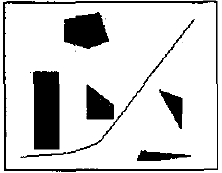
\includegraphics[width=\linewidth]{images/Chap1/R17_simple.png} % Replace with your figure
        \caption{Simple obstacle environment       }
        \label{Simple obstacle environment}
    \end{minipage}
    \begin{minipage}{0.30\textwidth}
        \centering
        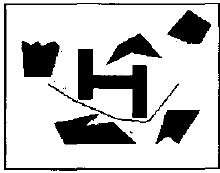
\includegraphics[width=\linewidth]{images/Chap1/R17_intermediate.png} % Replace with your figure
        \caption{Intermediate obstacle environment}
        \label{Intermediate obstacle environment}
    \end{minipage}
    \begin{minipage}{0.30\textwidth}
        \centering
        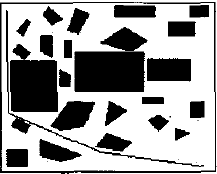
\includegraphics[width=\linewidth]{images/Chap1/R17_complex.png} % Replace with your figure
        \caption{Complex obstacle environment}
        \label{Complex obstacle environment}
    \end{minipage}
    \caption{GA Test scenarios \cite{R17}}
    \label{R17 test scenarios}
\end{figure}

\subsubsection {Local Path Planning}
Local path planning has as the role to make real-time decisions about how to move 
safely and efficiently in their surroundings. Unlike global path planning, which focuses on 
finding the best overall route from a starting point to a destination based on a static map, local path 
planning deals with navigating the environment directly around the robot while considering real-time
data input from sensors without prior knowledge about the surroundings\cite{R18}. This involves quickly 
responding to obstacles that appear or changes in the terrain, ensuring the robot can 
continue moving without collisions. Unlike Global Path planning, it functions without prior localization
and mapping of the surrounding environment. Local path planning is crucial for the safe and effective 
operation of robots, especially in 
dynamic and unkown environments. For example, in busy spaces with moving people 
or vehicles, a robot needs to be able to make quick adjustments to avoid accidents. This type of 
planning allows the robot to react immediately to new information, making it essential for applications 
where unpredictability and quick responses are vital, such as in autonomous vehicles or service robots in 
warehouses and factories.

Common Techniques involve Reactive methods which are approaches in local path planning that focus on real-time
obstacle avoidance and online adjustements on the path that are processed while the robot is navigating.
Techniques like the Potential Fields, 
Dynamic Window Approach (DWA), and Bug Algorithms are commonly used. In their research paper \cite{R25},
Buniyamin, N. et al. propose the point to point Bug algorithm to navigate in unkown environments. 
Bug algorithms are based on range sensors input. The robot at the starting point, plans to move directly to the 
target. Then it rotates scanning for obstacle points. If it encounters a sudden point, it navigates in its direction.
The robot rotates in the target's direction until it is able to resume its direct path to the target based on the 
constant search for the shortest distance from the current standpoint or find the next obstacle. 
While this approach is simple from the computational point of view and the hardware used, it may not be 
optimal considering other metrics.
Its path length optimality depends on the nature of the environments and its effciency decreases if the complexity
of the test area increases. 
Local path planning approaches are effective in navigating through cluttered environments, but when it comes to 
long-range planning, a hybrid approach that integrates both local and global path planning strategies can provide 
more robust and efficient results.

\subsubsection {Hybrid Path Planning}

In recent years, path planning approaches that combine both global and local techniques have gained popularity. 
By integrating global and local path planning approaches, robots and autonomous vehicles can take advantage of 
the strengths of both methods. This hybrid approach is a promising area of research, with the potential to benefit 
a wide range of applications. Hybrid path planning approaches are becoming increasingly popular due to their ability 
to handle complex environments and dynamic obstacles.

\noindent
\begin{minipage}{0.5\textwidth}  
    In \cite{R19}, Liu et al. used Djikstra ALgorithm for Global path planning and 
    the DWA as the local path planner for sudden unkown obstacles that could 
    appear for smart cars while following the global path.
    It works by evaluating different possible movements the robot could make within a short time frame 
    and choosing the one that avoids obstacles while also moving towards the goal. The "window" refers 
    to a limited set of possible velocities of the velocity space the robot can use based on its current 
    speed and capabilities. Figure \Ref{flowchart of the DWA} details the flowchart of the DWA. 
    The combined algorithms were tested on 3 spaces with 3 stages of environment complexity ranging from 
    simple to complex. The tests showed that the hybrid path planning approach was efficient for navigating the 
    robot and avoiding collisions. However, the tests were effected with dynamic obstacles only inside the simulation.
\end{minipage} 
\begin{minipage}{0.5\textwidth}  
    \centering  
    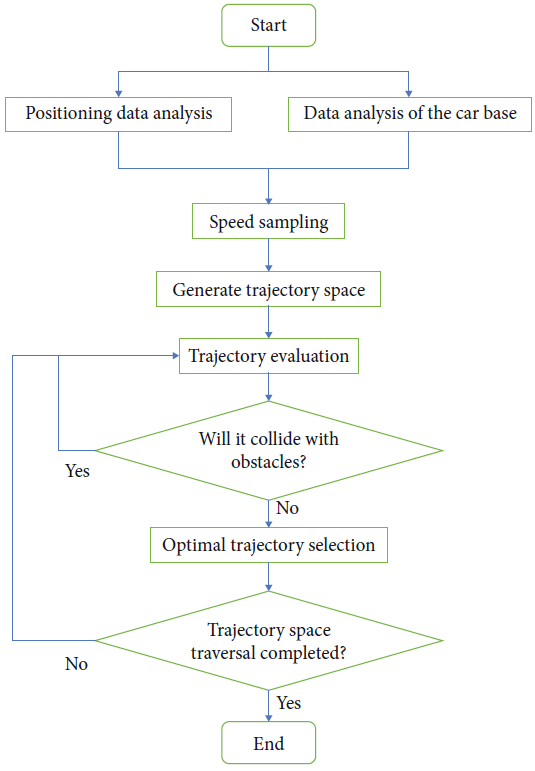
\includegraphics[width=\linewidth]{images/Chap1/DWA_flowchart.png}  
    \captionof{figure}{Flowchart of the DWA \cite{R19}}  
    \label{flowchart of the DWA}  
\end{minipage}  


Sensor-based approaches, on the other hand, rely on data collected by the robot's sensors, such as LIDAR, 
sonar, or cameras, to make decisions about where to go next. These sensors help the robot create a map of 
its surroundings, which can then be used to identify obstacles and safe paths. Occupancy grids and Point 
cloud processing are techniques used to interpret the sensor data and guide the 
robot's movements. This approach allows the robot to have a detailed understanding of its immediate 
environment, making it more capable of avoiding obstacles and navigating complex spaces.

\subsection{Discussion}

While traditional path planning methods have proven effective across various applications and usecases, 
they often face challenges when applied to highly structured, repetitive environments like those found 
in industrial automation. To overcome these limitations, the research in the previous years became rather 
oriented to investigating and using heuristic approaches. In \cite{R26}, Masehian et al. conducted a 
chronological review about the followe approaches in Motion Planning (MP). The results testify that in 30 years,
The application of Heuristic approaches in MP went from 0\% to 54\% from 1977 to 2007 as shown on Figure 
\Ref{heuristic barchart}.

\begin{figure}[H]
    \centering  
    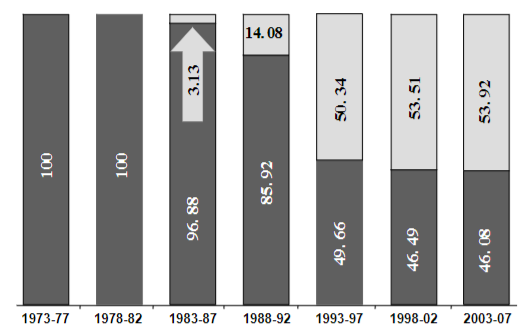
\includegraphics[width=3.5in]{images/Chap1/heuristic_barchart.png}\\ 
    \captionof{figure}{Application of classic and heuristic approaches in MP \cite{R26} 
    \newline \textbf{Dark gray:} Classic approaches
    \newline \textbf{Light gray:} Heuristic approaches }
    \label{heuristic barchart} 
\end{figure}

The classic algorithms have the drawback of traps in local minima and increased complexity in sophisticated environments.
In practice, the conditions where the robot operates are cluttered and complex than we can imagine which makes the classic 
approaches impractical. Consequently, it is necessary to tackle these issues in a different way. Although 
probabilistic methods proved high computational capabilities, scientists tend to combine 2 algorithms to 
benefit from the classic and heuristic advantages simultaneously. In \cite{R27}, Chen et al. delve into a hybrid
approach for online motion planning. Their approach is based on space exploration and heuristic search to determine 
optimal path linking a start point to an end goal. Tested on both low and high speed scenarios, the algorithm ensured
a low planning time: it outperformed RRT and had similar results in terms of planning time to Hybrid A*. 

To draw to a close, even though researches confirm that the heuristic approach prevails the classic one:
\cite{R20} and \cite{R25}, these approaches are not without their limitations. Heuristic methods, while good at 
navigating complex environments and avoiding local minima, sometimes fall short in finding the best possible 
solutions, especially in high-dimensional spaces. In contrast, classical methods, though computationally 
expensive, provide a more systematic and theoretically solid approach to path planning. To address these trade-offs, 
there is growing interest in hybrid methods that combine the strengths of both approaches. 
These hybrids use the precision and reliability of classical methods along with the flexibility and 
speed of heuristics. By doing so, they reduce the weaknesses of each approach, offering a more 
balanced and effective solution for path planning in complex environments. As a result, hybrid 
methods hold promise for future research, potentially leading to more efficient and dependable 
path planning algorithms.

\newpage
\section{Spline based Paths}
%introduction
This section will closely examine splines, their different types, their application in robotics and the 
importance of their integration and detail the challenges and limitations related to the use of Splines
for robotic motion planning, and conclude by a discussion around their relevance to this work.

\subsection{Definitions and Basic Concepts}

In mathematics and computer graphics, a \textbf{curve} is a continuous and smooth flowing line without sharp angles. 
It can be defined parametrically or implicitly and represents a path that can be traced by a moving point.
A curve can be defined using a parameter 
\(u\), where \(u\)varies over an interval, and the coordinates of the curve are given by functions of:
\begin{equation}
    C(u) = (x(u), y(u)) \quad \text{given} \quad a \leq u \leq b \label{eq:curve}
\end{equation}

The circle is an example of a curve where:

\hspace*{-1cm} % Adjust the value as needed
\begin{align}
    x(u) &= \cos(u) \\
    y(u) &= \sin(u) \quad \text{given} \quad 0 \leq u \leq \frac{\pi}{2}     \cite{R29}
\end{align}

whereas, the implicit form of the circle would be:
\begin{equation}
    (x - h)^2 + (y - k)^2 = r^2
\end{equation}

where \((h,k)\) is the center and \(r\) is the radius.


Parametric curves have a clear direction (from C(a) to C(b)), which implicit curves lack. This makes 
it simpler to create ordered sequences of points along a parametric curve. Additionally, the parametric 
form is more intuitive for designing and modeling shapes on a computer, as the coefficients in many 
parametric functions (such as Bezier and B-Splines) carry geometric significance. This results in 
user-friendly design techniques and algorithms that are numerically stable \cite{R28}. 
However, using one polynome-curves is inadequate as it is not possible to represent complex shapes, certain 
curve changes, and fitting the needed points. 
The solution is to use piecewise polynomial curves of degree \((n-1)\) for example if we need to integrate
\(n\) data points \cite{R29}.

Polynomials are a commonly used type of function in robotics because they can be easily differentiated 
and are less prone to numerical rounding errors (known as floating point errors). Although they cannot 
represent every geometric curve, polynomials can usually approximate them with sufficient accuracy.

Using classical polynomial functions or their derivatives in Bézier form is mathematically equivalent. 
This means that any curve described using standard polynomials can be transformed into a Bézier curve, 
and vice versa. However, when it comes to geometric modeling—especially in applications like computer 
graphics or robotics—the Bézier form is often preferred. This preference is due to the fact that the 
coefficients in the standard polynomial form (also known as the power basis form) don't offer much 
information about the curve's actual shape, making it harder to intuitively control and adjust the 
curve. In contrast, the coefficients in the Bézier form -the control points- directly influence the 
shape of the curve, in a visually meaningful way, making it easier to understand and manipulate 
as shown in equation \Ref{Bezier curve} \cite{R28}. 

\begin{equation}
    C(u) = \sum_{i=0}^{n} B_{i,n}(u) \mathbf{P}_i \quad \text{with } 0 \leq u \leq 1 \label{Bezier curve}
\end{equation}

The basis function \( B_{i,n}(u) \) is called the Bernstein polynomial of degree \( n \) and follows the equation

\begin{equation}
    B_{i,n}(u) = \frac{n!}{i!(n - i)!} \cdot u^i \cdot (1 - u)^{n - i} \label{}
\end{equation}

In this context, the Bernstein polynomial is a fundamental component. 
The basis function \( B_{i,n}(u) \) is used to determine how much influence each control 
point \( \mathbf{P}_i \) has on the shape of the Bézier curve.

The geometric coefficients \( \mathbf{P}_i \) are known as control points, and they define 
the shape of the polynomial curve. In many applications, such as mapping trajectories, 
a large number of control points is needed \cite{R28}.
Furthermore, in the Bézier form, the continuity of the curve depends on the placement of 
control points. This means if you want to change the shape of part of the curve while keeping 
the rest smooth, you can't easily do so because changing one part affects the whole curve \cite{R29}.

Instead, a more effective curve representation can be expressed as:

\begin{equation}
    C(u) = \sum_{i=0}^{n} N_i(u) \mathbf{P}_i
\end{equation}

where:
\begin{itemize}
    \item \( \mathbf{P}_i \): the control points
    \item \( N_i(u) \): the piecewise polynomial functions
\end{itemize}
The continuity of the curve is determined by these basis functions, allowing for flexible modification of 
control points without affecting the curve's smoothness \cite{R29}.

The basis functions for B-splines are defined recursively. For a given degree \( p \) and a set of non-decreasing knot values 
\( \{ u_i \} \), the basis functions \( N_{i,p}(u) \) can be defined as:

\begin{equation}
    N_{i,0}(u) = 
\begin{cases} 
1 & \text{if } u_i \leq u < u_{i+1} \\
0 & \text{otherwise}
\end{cases}
\end{equation}

\begin{equation}
N_{i,p}(u) = \frac{u - u_i}{u_{i+p} - u_i} N_{i,p-1}(u) + \frac{u_{i+p+1} - u}{u_{i+p+1} - u_{i+1}} N_{i+1,p-1}(u)
\end{equation}


With:
\begin{itemize}
    \item \( u \) is the parameter along the curve.
    \item \( u_i \) are the knot values, which divide the parameter range into intervals.
    \item \( N_{i,p}(u) \) are the B-spline basis functions of degree \( p \).
\end{itemize}

In figure \Ref{NURBS} stands an example of a NURBS spline generated through setting random 
control points using th NURBS generator \cite{R32}

\begin{figure}[H]
    \centering
    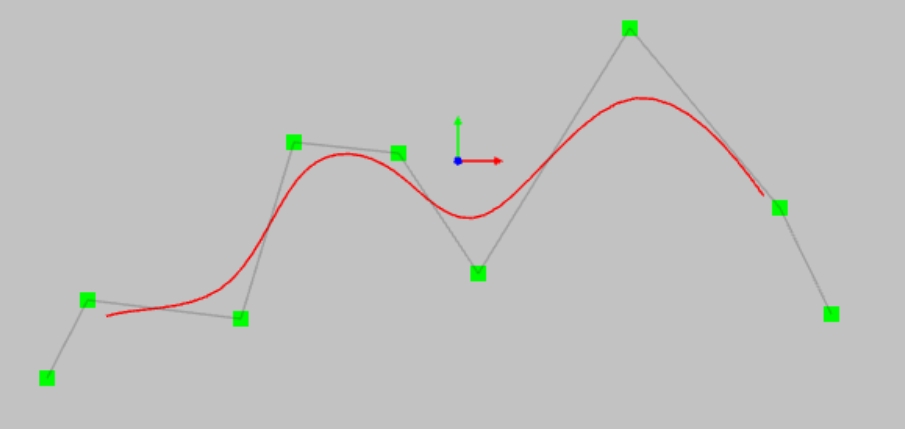
\includegraphics[width=4in]{images/Chap1/control-spline.png}
    \caption{NURBS spline example
    \newline \textbf{Green}: Control points
    \newline \textbf{Red}: NURBS spline}
    \label{NURBS} 
\end{figure}

Understanding these principles is essential as we move forward to explore the applications of splines 
in robotics. In the next section, we will examine how these spline concepts are applied to solve 
real-world problems in robotic path planning and motion control.

\subsection{Applications of Splines in Robotics}
\subsubsection{Trajectory Planning} 
%How splines facilitate smooth and continuous trajectory planning.
Robots like AMRs in the intralogistics sector usually have mission to carry heavy loads. 
This property makes it risky to operate abrupt motion changes like stopping or turning.
These vehicles' motion planning requires precise control and detailed alignment to the 
kinematic constraints that they present \cite{R30}.
Given the mathematical nature of B-Splines, they ensure continuity of the first and second derivatives.
This continuity translates to smooth transitions of the resulting velocities and accelerations of the path
that the robot will follow. By having continuous velocity and acceleration, we make sure that the robot
achieves smooth transitions and speed changes. Furthermore, tracking, precise following and correct control
interventions are guaranteed allowing for precise navigation \cite{R30}. 

 
Although simple,
the connected waypoints approach comes with drawbacks like sub-optimal travel time, unoptimized long paths, 
and mechanical wear because of abrupt direction changes unlike curved paths \cite{R30}. The morphological 
difference in both paths is distinguished in figure \Ref{paths} 

\begin{figure}[H]
    \begin{center}
        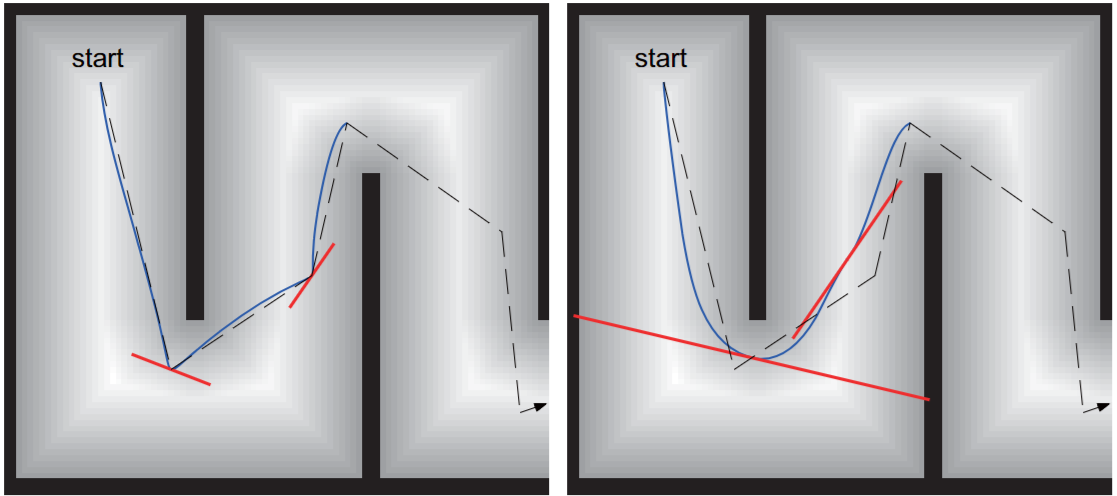
\includegraphics[width=4in]{images/Chap1/sharp-vs-curved-path.png}\\
        \caption{Morphological difference between a path connecting waypoints (left) and a curved path 
        (right) \cite{R30}}
        \label{paths}
    \end{center}
\end{figure}

Multiple approaches have been developed to introduce smooth transitions and turns into robot trajectories. 
One such method involves using Clothoid curves, which connect straight path segments with circular arcs 
to avoid abrupt changes in direction \cite{R31}. Originally introduced for designing highways and roads to 
ensure safe and comfortable driving for humans, Clothoids offer a gradual change in curvature.

However, when applied to robotics, Clothoid curves present certain drawbacks. These include the potential 
for discontinuities in curvature at the transitions, which can lead to jerky motions in robotic paths. 
Additionally, Clothoid-based paths can result in sub-optimal path lengths, as they may not be the shortest 
possible routes. Moreover, while circular arcs with constant radii are used in this approach, longer 
arcs lead to larger curvatures, which can be impractical for mobile robots that require tighter turns 
and more precise control \cite{R31}.

%Techniques for smoothing rough paths generated by planners.
Migrating from a path with sharp angles to one with smooth curves can be effectively accomplished by 
using splines. The interpolation of the control points of the original path 
creates a smooth, continuous curve. By incorporating a convex hull around these control points, we 
ensure that the path does not deviate excessively from the desired points, thus avoiding potential 
collisions with obstacles \cite{R33}. The convex hull acts as a boundary that keeps the spline inside the limits of 
the control points that prametrize it (see figure \Ref{convex-hull}) and keeps the robot from straying 
too far, ensuring a safe and accurate trajectory \cite{R29}.

\begin{figure}[H]
    \begin{center}
        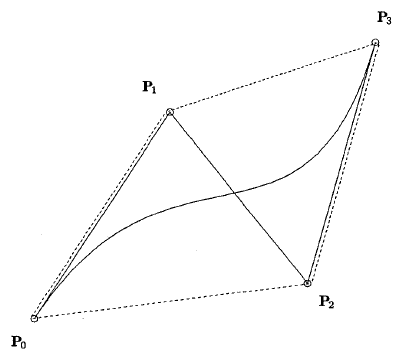
\includegraphics[width=3in]{images/Chap1/convex-hull.png}\\
        \caption{Convex hull contained Spline \cite{R29}}
        \label{convex-hull}
    \end{center}
\end{figure}

Splines are advantageous because they can accommodate various constraints such as curvature limits 
and minimum turning radii. These constraints are crucial in many applications, including robotics 
and vehicle navigation, where maintaining a smooth path is essential for stability and control. 
By adjusting the spline parameters, it is possible to design paths that meet specific requirements, 
ensuring that the resulting trajectory is not only smooth but also feasible given the physical and 
operational constraints \cite{R30}.

In scenarios involving obstacle avoidance, splines can be blended or connected to create a seamless 
path while circumventing obstacles. This blending technique allows for the integration of different 
spline segments into a continuous trajectory, ensuring that the path remains clear of obstacles. 
By carefully adjusting the blend points and ensuring smooth transitions between splines, it is 
possible to navigate complex environments safely and efficiently. This approach combines the 
advantages of smooth path planning with effective obstacle avoidance.

%Case studies of spline-based trajectory planning in autonomous vehicles.

A notable case study of splines integration in solving path planning problems, is a research conducted 
by B. Lau et al. \cite{R30} that aims to develop a time optimal solution while considering the kinodynamic 
properties of a mobile robot. They used a global planner to generate straight-line paths and minimize time 
of travel. Then, they  integrated splines to join the resulting path segments in a smooth and continuous 
way and replan in case of unprecedented collisions. The results show that our motion planning system works 
well in both real and simulated settings. It created smooth and accurate paths, with an average positional 
error of about 1 cm and a velocity error of less than 2 cm/s. The optimization process improved travel 
time by 31\% compared to initial paths. The system also handled dynamic environments, like crowded trade 
shows, and adjusted smoothly when localization errors occurred by updating the path as needed. Overall, 
it performed reliably, navigating precisely and adapting effectively to changes and errors.

\subsection{Discussion}
In general, Splines are an effective tool that centralizes advantages related to path smoothness, 
simplicity of constraining the path according to the kinodynamic properties and mechanical limitations of the 
mobile robot like limiting the curvature, and allowing for safe and smooth speed and direction changes. 
These properties accommodate simple manipulation of splines for path planning and tracking of path properties.
As an illustration, it is possible to measure the spline's features like curvature or approximate its length.
Figure \Ref{curvature}, shows an example plot of the curvatures of 3 random splines.

\begin{figure}[H]
    \begin{center}
        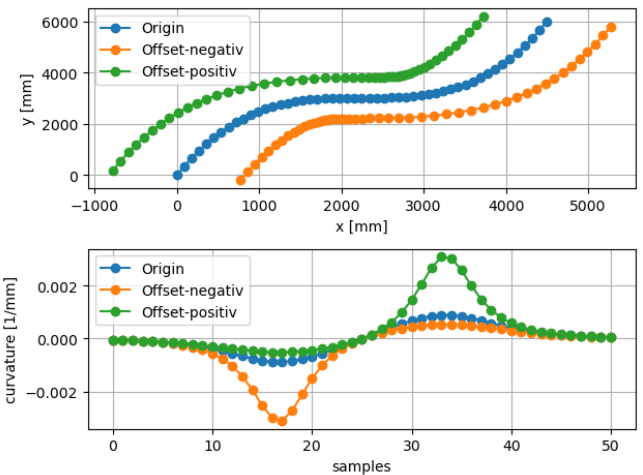
\includegraphics[width=3.5in]{images/Chap1/curvature.png}\\
        \caption{Curvature of 3 S-shaped splines}
        \label{curvature}
    \end{center}
\end{figure}
In the next section, we discuss the ways we can use such information about the splines to measure paths quality.

\section{Metrics}
\section{Optimization Techniques}








